\documentclass[12pt,a4paper,twoside]{book}
\usepackage{graphicx}
\usepackage{setspace}	%double spacing for text, single for captions, footnotes, etc.
%\usepackage{hypernat} 	%substitut de cite que permet fer hyperlinks
\usepackage{natbib}		% substituye a 'hypernat' que funciona en Windows.
\usepackage[spanish]{babel}
\usepackage[utf8]{inputenc}
\usepackage{color}
\usepackage{hhline} 		% extended styles for tables
\usepackage{multirow}
\usepackage{subfigure}
\usepackage{acronym}
\usepackage{hyperref}
\usepackage{amsmath,amsmath,amssymb} 
\usepackage{fancyhdr}
\usepackage{epsfig, amsmath}
\usepackage{algorithm}
\usepackage{algorithmic}

% general settings
\hypersetup{
	linktocpage=true,
	colorlinks=true,
	linkcolor=blue,
	citecolor=blue,
}
\definecolor{Hgray}{gray}{0.6}

\newenvironment{definition}[1][Definition]{\begin{trivlist}
\item[\hskip \labelsep {\bfseries #1}]}{\end{trivlist}}

\setlength{\topmargin}{0cm}
\setlength{\textheight}{23cm}
\setlength{\textwidth}{17cm}
\setlength{\oddsidemargin}{0cm}
\setlength{\evensidemargin}{0cm}
\setlength{\headheight}{1cm}

% indica que las 'sub-sub-sections' sean numeradas y aparezcan en el indice
\setcounter{secnumdepth}{3}
\setcounter{tocdepth}{2}

% settings for code
\renewcommand{\algorithmicrequire}{\textbf{Entrada: }}
\renewcommand{\algorithmicensure}{\textbf{Salida: }}

%%%%%%%%%%%%
% DOCUMENT %
%%%%%%%%%%%%
\begin{document}

% portada
\newpage
\thispagestyle{empty}

\baselineskip 2em

%\vspace*{1cm}

\centerline{
\includegraphics[width=0.6\textwidth]{images/UOC-logo}}
\begin{center}
\textsc{Universitat Oberta de Catalunya (UOC) \\
 Máster Universitario en Ciencia de Datos (\textit{Data Science})\\}

%\centerline {\pic{UOC}{4cm}}

\vspace*{1.5cm}

\textsc{\Large TRABAJO FINAL DE MÁSTER}

\vspace*{0.5cm}

\textsc{\large Área: PLN}


%\textbf{\Huge VirtualTechLab Model: }

\vspace*{2.0cm}

\textbf{\Large Modelización de temas de llamadas en tiempo real}

\textbf{\large PEC II}

\vspace{2.5cm}
\baselineskip 1em

\baselineskip 2em
-----------------------------------------------------------------------------\\
Autor:      Manuel E. Gómez Montero\\
Tutora UOC:      Ana Valdivia Garcia\\
Tutor TE:      Antonio Fernández Gallardo\\
Profesor:   Jordi Casas\\
-----------------------------------------------------------------------------\\
\vspace*{1.5cm}
Madrid, \today

\end{center}

\newpage
\pagestyle{empty}
\hfill

\newpage
% abstract
\pagenumbering{roman} 
\setcounter{page}{1} 
\pagestyle{plain}

%%%%%%%%%%%%%%%%
%%% CREDITOS %%%
%%%%%%%%%%%%%%%%
%\chapter*{Créditos/Copyright}

%Una página con la especificación de créditos/copyright para el proyecto (ya sea aplicación por un lado y documentación por el otro, o unificadamente), así como la del uso de marcas, productos o servicios de terceros (incluidos códigos fuente). Si una persona diferente al autor colaboró en el proyecto, tiene que quedar explicitada su identidad y qué hizo.

%A continuación se ejemplifica el caso más habitual, aunque se puede modificar por cualquier otra alternativa:

%\vspace{1cm}

%\begin{figure}[ht]
%    \centering
%	
\includegraphics[scale=1]{images/license.png}
%\end{figure}

%Esta obra está sujeta a una licencia de Reconocimiento -  NoComercial - SinObraDerivada

%\href{https://creativecommons.org/licenses/by-nc-nd/3.0/es/}{3.0 España de CreativeCommons}.

%%%%%%%%%%%%%
%%% FICHA %%%
%%%%%%%%%%%%%
%\chapter*{FICHA DEL TRABAJO FINAL}

%\begin{table}[ht]
%	\centering{}
%	\renewcommand{\arraystretch}{2}
%	\begin{tabular}{r | l}
%		\hline
%		Título del trabajo: & Descriptivo del trabajo\\
%		\hline
%       Nombre del autor: & Nombre y dos apellidos\\
%		\hline
%        Nombre del colaborador/a docente: & Nombre y dos apellidos\\
%		\hline
%        Nombre del PRA: & Nombre y dos apellidos\\
%		\hline
%        Fecha de entrega (mm/aaaa): & MM/AAAA\\
%		\hline
%        Titulación o programa: & Plan de estudios\\
%		\hline
%        Área del Trabajo Final: & El nombre de la asignatura de TF\\
%		\hline
%        Idioma del trabajo: & Catalán, español o inglés\\
%		\hline
%        Palabras clave & Máximo 3 palabras clave\\
%		\hline
%	\end{tabular}
%\end{table}

%%%%%%%%%%%%%%%%%%%
%%% DEDICATORIA %%%
%%%%%%%%%%%%%%%%%%%
%\chapter*{Dedicatoria/Cita}

%Breves palabras de dedicatoria y/o una cita.

%%%%%%%%%%%%%%%%%%%
%%% Agradecimientos %%%
%%%%%%%%%%%%%%%%%%%
%\chapter*{Agradecimientos}



%%%%%%%%%%%%%%%%
%%% RESUMEN  %%%
%%%%%%%%%%%%%%%%
\chapter*{Resumen}
\addcontentsline{toc}{chapter}{Abstract}


Un call-center es el área de una empresa el cuál se encarga de recibir y transmitir llamadas desde o hacia clientes, socios comerciales u otras compañías externas. Debido a la gran cantidad de información que se transfiere en estos centros, resulta una tarea esencial optimizar el tiempo de respuesta para así reaccionar en tiempo real a las peticiones de los clientes y mejorar la percepción que estos tienen sobre la compañía. 

Una manera de mejorar el rendimiento es detectar el tema de las llamadas  mediante técnicas de \textit{machine learning} dando la posibilidad a la empresa de reaccionar en tiempo real, en función de la temática que se este tratando en cada momento. 



%El documento que se presenta tiene como objetivo final mejorar la operatividad del \textit{call-center}  de una gran empresa, extrayendo mediante técnicas de \textit{machine learning} la temática de las llamadas que se realizan al mismo y dando la posibilidad a la empresa de reaccionar en tiempo real, en función de la temática que se este tratando en cada momento. 

El sistema que se presenta en el documento nos permite, a partir de la transcripción de las llamadas al \textit{call-center} de Telefónica España, descubrir en tiempo real la temática de las mismas. Esta modelización de \textit{topics} se ha realizado utilizando métodos de Procesamiento de Lenguaje Natural y aprendizaje profundo. El sistema realiza la clasificación de las nuevas llamadas en tiempo real, permitiendo a los usuarios visualizar la evolución en la temática de las mismas y generar alertas en base a anomalías.  


%TODO Es un borrador volver al  resumen una vez acabado el proyecto.
\onehalfspacing

\vspace{1.5cm}

\textbf{Palabras clave}: ``natural language processing'', ``sentiment analysis'', ``real time'', ``call center'', ``topic modeling'', ``deep learning''
\newpage

\pagestyle{fancy}
\renewcommand{\chaptermark}[1]{ \markboth{#1}{}}
\renewcommand{\sectionmark}[1]{\markright{ \thesection.\ #1}}
\lhead[\fancyplain{}{\bfseries\thepage}]{\fancyplain{}{\bfseries\rightmark}}
\rhead[\fancyplain{}{\bfseries\leftmark}]{\fancyplain{}{\bfseries\thepage}}
\cfoot{}

% indice
\cleardoublepage
\phantomsection
\addcontentsline{toc}{chapter}{Índice}
\tableofcontents
% listado de figuras
%\cleardoublepage
%\phantomsection
%\addcontentsline{toc}{chapter}{Llistado de Figuras}
%\listoffigures
% listado de tablas
%\cleardoublepage
%\phantomsection
%\addcontentsline{toc}{chapter}{Listado de Tablas}
%\listoftables

\thispagestyle{empty}

\pagenumbering{arabic}

\pagestyle{fancy}
\renewcommand{\chaptermark}[1]{ \markboth{#1}{}}
\renewcommand{\sectionmark}[1]{\markright{ \thesection.\ #1}}
\lhead[\fancyplain{}{\bfseries\thepage}]{\fancyplain{}{\bfseries\rightmark}}
\rhead[\fancyplain{}{\bfseries\leftmark}]{\fancyplain{}{\bfseries\thepage}}
\cfoot{}

\onehalfspacing

% capitulos del documento
\chapter{Introducción}
\label{chapter:introduccion}

Este primer capítulo del trabajo tiene como objetivo presentar, a grandes rasgos, la propuesta (sección \ref{section:intro:descripcion}), los objetivos que pretendemos lograr (sección \ref{section:intro:objetivos}), la motivación que nos ha llevado a abordar este proyecto (sección \ref{section:intro:motivacion}) y un repaso a las tareas que serán necesarias para la ejecución del mismo (sección \ref{section:intro:planificacion}). 


\section{Descripción general de la propuesta}
\label{section:intro:descripcion}
En los últimos años, la explosión ingente en la generación de datos y el avance en las capacidades tecnológicas que nos permiten recolectar, almacenar y procesar los datos generados; han provocado que empecemos a abordar el estudio de otro tipo de datos no estructurados que antes no se podían analizar como imágenes, textos, audios, etc. Como resultado, diferentes áreas del conocimiento (Procesamiento del Lenguaje Natural, Análisis de Imágenes) han experimentado un creciente interés tanto en la comunidad científica como en el mundo de los negocios. 


Dentro de los datos no estructurados, una de las fuentes de información con mayor potencial en todas las grandes empresas que prestan servicio al público general, son las llamadas que los clientes realizan a su \textit{call-center}, ya que nos permiten obtener una idea de la percepción que los clientes tienen de nuestra empresa y de sus preocupaciones en cada momento. 

La propuesta que pretendemos abordar en este trabajo consiste en extraer la temática de  estas llamadas en el momento en el que son capturadas. Aunque actualmente esta captura se hace periódicamente pretendemos construir una solución que nos permita el tratamiento de las mismas en tiempo real o streaming, y de esta manera mejorar el rendimiento de estos centros. %para que esta solución sea válida en un futuro próximo cuando se aumente la frecuencia de ingesta. 

Esta extracción en tiempo real nos permitirá conocer cómo evolucionan los temas que tratan nuestros clientes cuando llaman a nuestro \textit{call-center} para así poder reaccionar inmediatamente ante una preocupación concreta. 


\section{Motivación}
\label{section:intro:motivacion}
La motivación que nos ha llevado a acometer un proyecto de esta naturaleza viene originada por diferentes factores que están ligados tanto al negocio como a las capacidades técnicas disponibles en la empresa. 

Por un lado, la capacidad de obtener la temática de las llamadas en tiempo real se presenta como una oportunidad de mejorar la operatividad de un \textit{call-center} y por ende la satisfacción de los clientes, permitiéndonos entenderlos mejor y así reaccionar de una manera ágil a sus necesidades reales.

Desde el punto de vista técnico, también es el momento ideal para emprender este proyecto debido tanto a la disponibilidad periódica de transcripciones de las llamadas, que nos permiten ahorrarnos el paso de realizar un \textit{Speech 2 Text} para obtener nuestro conjunto de datos; como al aumento de capacidades técnicas en la empresa que nos permitirán tanto entrenar nuestros modelos, como poder tratar y explotar los datos en tiempo real. 


\section{Objetivos}
\label{section:intro:objetivos}
En este apartado definiremos los objetivos que se pretenden conseguir con este proyecto. Estos objetivos deben ser \textit{SMART}, es decir: 

\begin{itemize}
	\item \textit{\textbf{S}pecific}: Deben plantearse de una forma detallada y concreta.
	\item \textit{\textbf{M}easurable}: Deben poder medirse con facilidad.
	\item \textit{\textbf{A}chievable}: Deben ser objetivos realistas.
	\item \textit{\textbf{R}elevant}: Tienen que ser relevantes para la empresa y ofrecernos un beneficio claro.
	\item  \textit{\textbf{T}imely}: Estos objetivos tienen que tener un tiempo establecido.
\end{itemize}




El objetivo general es optimizar el proceso de atención de llamadas en el call-center mediante técnicas de Procesamiento del Lenguaje Natural y Aprendizaje Profundo. Concretamente, los objetivos específicos que se pretenden conseguir con este proyecto son: 

\begin{itemize}
	\item \textbf{Construir un modelo que nos permita extraer la temática de las llamadas} a partir de su transcripción a texto. Este objetivo debemos alcanzarlo en la fase de modelado y podremos medir su éxito atendiendo al porcentaje de llamadas que podamos clasificar correctamente en un proceso de test. Se trata del objetivo principal del proyecto.
	\item Desarrollar un mecanismo que nos permita \textbf{extraer esta temática para nuevas llamadas en tiempo real}. De este modo tendremos un sistema vigente cuando la frecuencia en la recepción de las llamadas aumente. Este objetivo se deberá alcanzar en la fase de productivización. 
	\item Disponer de una\textbf{ visualización en tiempo cuasi real} para que pueda visualizarse la evolución de las temáticas a lo largo del tiempo. Este objetivo se deberá alcanzar en la fase de productivización. 
	\item Proporcionar un \textbf{sistema de alertado} que nos permita detectar anomalías en el número de llamadas que se reciben de un determinado tema. Este objetivo se deberá alcanzar en la fase de productivización.
\end{itemize}

En las conclusiones de este proyecto se evaluará el éxito o fracaso del mismo en función del grado de cumplimiento de estos objetivos.

\section{Tareas y planificación}
\label{section:intro:planificacion}
El proyecto se llevará a cabo desde el 16 de Septiembre hasta el 20 de Febrero. Para poder abordar la ejecución del  mismo se han extraído las siguientes tareas principales: 


\begin{figure}[!ht]
	\centering
	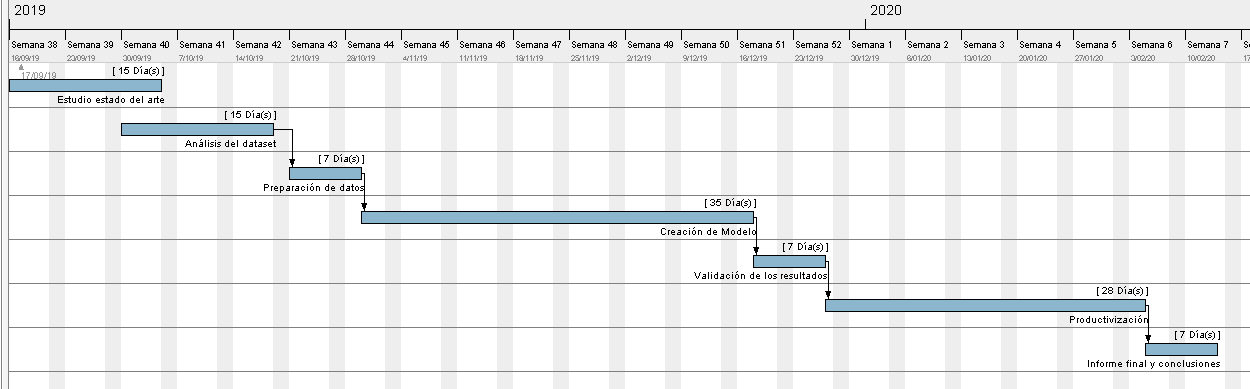
\includegraphics[width=\textwidth]{images/intro/gantt}
	\caption{Diagrama de Gantt}
	\label{fig:gantt}
\end{figure}


\begin{itemize}
	\item \textbf{Estudio estado del arte}: En esta fase se realizará una prospección para conocer el estado del arte en todos los puntos relacionados con el proyecto: Procesamiento del Lenguaje Natural, tecnologías de tratamiento de datos en tiempo real y \textit{Big Data}. 
	
	\item \textbf{Análisis del \textit{dataset}}: El propósito de esta tarea es entender el \textit{dataset}  y estudiar las posibilidades del mismo. 
	
	\item\textbf{ Preparación del \textit{dataset}}: Una vez realizado el estudio del \textit{dataset} es necesario realizar labores de limpieza y transformación de los datos de modo que estos datos sean válidos para nuestro objetivo.
	
	\item \textbf{Creación del modelo}: En esta fase se procederá a la creación de un modelo capaz de obtener los temas de los que habla una determinada llamada. Este modelo será el \textit{core} de nuestro proyecto.
	
	\item \textbf{Validación de los resultados}: Una vez entrenado el modelo será necesario validar los resultados obtenidos para poder evaluar la bondad de nuestro modelo. 
	
	\item\textbf{ Productivización}: El trabajo no acaba con la creación de un buen modelo que nos permita extraer los temas de nuestras llamadas. Este modelo tendrá que ser puesto en producción y permitir al usuario final extraer los temas de las llamadas en tiempo real y darle la opción de crear alarmas basadas en la variación del número de eventos (llamadas) de un determinado tema.
	\item\textbf{ Informe final y conclusiones}: Por último, una vez llevado a a producción nuestro modelo, se realizará un informe final donde, entre otros puntos, se evaluarán los resultados obtenidos y se extraerán conclusiones y pasos futuros.
\end{itemize} 

\begin{figure}[!ht]
	\centering
	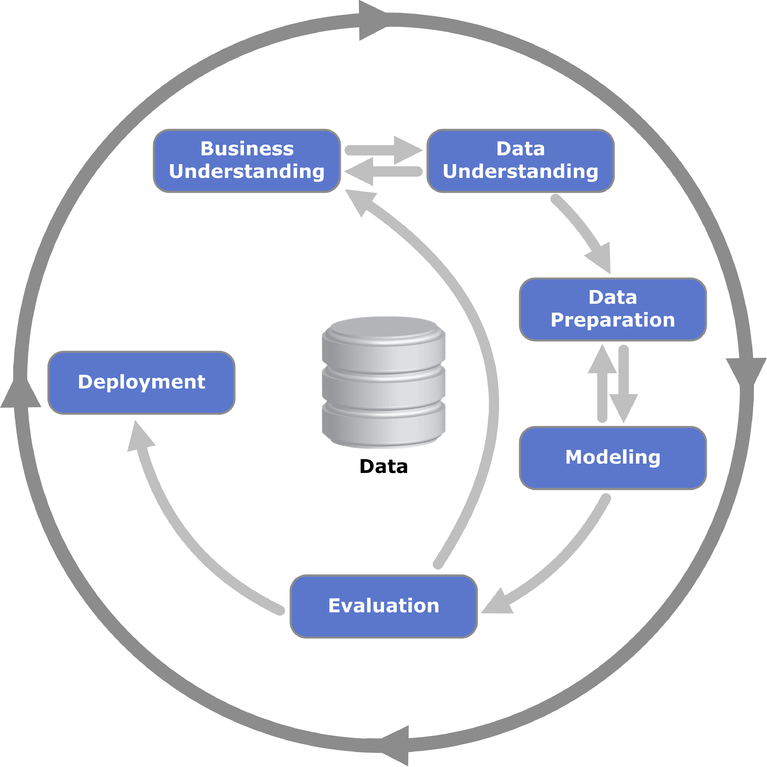
\includegraphics[width=0.63\textwidth]{images/intro/crispdm}
	\caption{Fases del modelo CRISP-DM}
	\label{fig:crispdm}
\end{figure}


Estas fases están basadas en el estándar \textbf{\textit{CRISP-DM}} (\cite{crispdm}), añadiendo una última tarea para nuestro informe final, \textit{CRISP-DM} nos proporciona una descripción del ciclo de vida de los proyectos de minería de datos de un modo bastante similar al que se aplica en los modelos de ciclo de vida de desarrollo \textit{software}.


 

En la Figura \ref{fig:crispdm} se observa el diseño de este modelo y cómo representa el ciclo de vida de un proyecto de minería de datos. En la imagen podemos ver en primer lugar un círculo exterior que refleja la naturaleza cíclica de los proyectos de minería de datos, además vemos cómo la secuencia de tareas no es rígida, pudiendo saltar hacia adelante o atrás entre tareas. En la gráfica se representan mediante flechas las dependencias más importantes y usuales entre tareas.

En nuestro desarrollo usaremos este modelo, aunque en el diagrama de la Figura \ref{fig:gantt} aparezca una secuencia de tareas más rígida, será usual, por ejemplo, el salto recíproco entre las fases de preparación de los datos y creación del modelo.



%\chapter{Estado del Arte}
\label{chapter:estadoarte}


El objetivo de este apartado es hacer un recorrido por el estado del arte relacionado con el proyecto, este recorrido lo enfocaremos desde tres puntos de vista diferentes:
\begin{itemize}
	\item \textbf{Procesamiento del Lenguaje Natural}: En este apartado nos centraremos en el procesamiento del lenguaje natural y su evolución a lo largo del tiempo. 
	\item \textbf{\textit{Deep Learning} y aplicación al Procesamiento del Lenguaje Natural}: En la segunda parte pondremos foco en el \textit{Deep Learning}, sus ventajas y cómo se están aplicando estos métodos al procesamiento de lenguaje natural. 
	\item \textbf{\textit{Big Data} y \textit{Fast Data}}: Por último, haremos un repaso a la evolución del \textit{Big Data} y cómo la tendencia actual es realizar el procesamiento en tiempo real mediante \textit{Fast Data}.
\end{itemize}

\section{Procesamiento de lenguaje natural}

\subsection{Historia}

Para hablar de los orígenes del procesamiento del lenguaje natural (a partir de ahora NLP por sus siglas en inglés \textit{Natural Lenguage Processing}) tal y como lo conocemos, tendríamos que remontarnos a los años 50, concretamente al artículo ``\textit{Computing Machinery and Intelligence}'' escrito por Alan Turing \cite{turing_1950}. En este artículo aparece el NLP dentro del campo de la inteligencia artificial y se presenta por primera vez el conocido ``Test de Turing`''. Este test convirtió la pregunta abstracta de ``¿Son capaces de pensar las máquinas?'' en un juego llamado: ``\textit{The Imitation Game}''. El juego propuesto inicialmente, de forma muy resumida, consiste en ver si una persona (interrogador) interrogando a dos personas (un hombre y una mujer), era capaz de descubrir el sexo de cada una; la modificación del mismo sustituye las dos personas de distinto sexo por una persona y una máquina y el interrogador debe ser capaz de descubrir si las preguntas están siendo respondidas por un humano o una máquina. En el caso de que no sepa discernir, la computadora gana la partida. Podemos encontrar más información al respecto en el libro \cite{turing}.



A partir de los avances de Turing y hasta los 80 el crecimiento en el campo del NLP se produjo principalmente con la creación de complejos sistemas basados en reglas escritas a mano. Fue en esta década cuando empezamos a vivir la incorporación de algoritmos de \textit{machine learning} enfocados al procesamiento del lenguaje natural. Este hecho se vio motivado principalmente por el increíble avance en la capacidad de cómputo, ya predicho por la ley de Moore, y por la aplicación de teorías ya existentes como los trabajos de Chomsky. 


Desde el comienzo de la aplicación de modelos de \textit{machine learning}, y de nuevo motivados por el crecimiento de la capacidad computacional de los sistemas actuales, se ha pasado de utilizar árboles de decisión, que creaban de manera automática reglas similares a las que se venían creando manualmente, a los modelos de \textit{deep learning} que están en auge en la última década. 

\subsection{Aplicaciones}

En el apartado anterior hicimos referencia a ``\textit{The Imitation Game}'' como inicio de lo que hoy conocemos como procesamiento de lenguaje natural, sin embargo, las aplicaciones en este campo han crecido de forma vertiginosa en estos 70 años, principalmente en las últimas décadas. Hoy en día, si tuviéramos que contestar a la pregunta: ``¿son capaces de pensar las máquinas?'', implicaría algo más que superar el test de Turing. Mirando a nuestro alrededor nos encontraríamos con asistentes de voz como Alexa o Siri que no solo contestan a nuestras preguntas, si no que realizan un trabajo de pasar nuestra voz a texto (\textit{Speech to Text}) y de nuevo el texto resultante a voz (\textit{Text to Speech}). Nos encontraríamos también con sistemas capaces de realizar traducciones simultáneas, otros capaces de autocompletar textos, de identificar preguntas y respuestas, de clasificar textos de acuerdo a temas o autores, incluso de analizar sentimientos positivos o negativos teniendo como entrada un texto u opinión... 


Según \cite{goldberg_2017} todos estos problemas tan diversos podríamos clasificarlos según en el punto del análisis que nos centremos: 

\begin{itemize}
	\item \textbf{Análisis de palabras}: En este tipo de problemas se pone foco en las palabras, como pueden ser ``perro'', ``hablar'', ``piedra'' y necesitamos decir algo sobre ellas. Por ejemplo: ``¿estamos hablando de un ser vivo?'', ``¿a qué lenguaje pertenece?'', ``¿cuáles son sus sinónimos o antónimos?''. Actualmente este tipo de problemas son menos frecuentes, ya que normalmente no pretendemos analizar palabras aisladas sino que es preferible basarse en un contexto. 
	
	\item \textbf{Análisis de textos}:  En este tipo de problemas no trabajamos solo con palabras aisladas, sino que disponemos de una pieza de texto que puede ser una frase, un párrafo o un documento completo y tenemos que decir algo sobre él. Por ejemplo: ``¿se trata de spam?'', ``¿qué tipo de texto es?'', ``¿el tono es positivo o negativo?'', ``¿quién es su autor?''.Este tipo de problemas son muy comunes y nos vamos a referir a ellos como \textbf{problemas de clasificación de documentos}.   
	
	\item \textbf{Análisis de textos pareados}: En esta clase de análisis disponemos de  dos textos (también podrían ser palabras aisladas) y tenemos que decir algo sobre ellos. Por ejemplo, ``¿los textos son del mismo autor?'', ``¿son pregunta y respuesta?'', ``¿son sinónimos?'' (para el caso de palabras aisladas).
	
	\item \textbf{Análisis de palabras en contexto}: En estos casos de uso, a diferencia del primer análisis que trataba unicamente con  palabras aisladas, tenemos que clasificar una palabra en particular en función del contexto en el que se encuentra. 
	
	\item \textbf{Análisis de relación entre palabras}: Este último tipo de análisis tiene como objetivo deducir la relación entre dos palabras existentes en un documento. 
	
\end{itemize}

Dependiendo del problema que queramos abordar usaremos un tipo de características del lenguaje u otro, por ejemplo, es usual que si estamos analizando palabras aisladas nos centremos en las letras de una palabra, sus prefijos o sufijos, su longitud, la información léxica extraída de diccionarios como \textit{WordNet} \cite{wordnet}, etc. En cambio, si estamos trabajando con texto, lo normal es que nos fijemos en otros conceptos estadísticos como el histograma de las palabras dentro del texto, ratio de palabras cortas vs largas, número de veces que aparece una palabra en un texto comparado con el resto de textos...  

El proyecto que se presenta en este documento está centrado en el análisis de textos, concretamente en extraer los temas de un documento (o llamada). Este tipo de problemas se conoce como modelización de \textit{topics}. 

En el siguiente punto de este apartado nos centraremos en algunos modelos y avances en este área que puedan servirnos de apoyo para nuestro proyecto. 


\subsection{Modelización de temas}
La modelización de topics hace referencia a un grupo de algoritmos de \textit{machine learning} que infieren la estructura latente existente en un grupo de documentos. 

Aunque la mayoría de los algoritmos de modelización son no supervisados, al igual que los algoritmos tradicionales de \textit{clustering}, existen también algunas variantes supervisadas que necesitan disponer de documentos etiquetados. 

Quizás el algoritmo más conocido para la modelización de topics sea el \textit{Latent Dirichlet Allocation} (normalmente conocido por su acrónimo, LDA). LDA fué presentado en 2003 en el artículo \cite{Blei_LDA}. Este algoritmo no supervisado asume que cada documento es una distribución probabilística de \textit{topics} y cada \textit{topic}, a su vez, es una distribución de palabras del documento. LDA usa una aproximación llamada ``\textit{bag of words}'', en la que cada documento es tratado como un vector con el conteo de las palabras que aparecen en el mismo. La principal característica de LDA es que la colección de documentos comparten los mismos topics, pero cada documento contiene esos topics en una proporción diferente. 


A partir de LDA surgieron numerosas variantes que repasaremos de forma breve, por ejemplo, en el mismo año de la creación de LDA y también presentado por los mismos autores en \cite{Blei_HTM}, surgió una \textbf{variante jerárquica} que permitía representar los \textit{topics} jerarquicamente. En 2006 en \cite{Blei_DTM} se desarrolla un modelo LDA dinámico denominado DTM (\textit{Dinamic Topic Model}), en el que se introduce la variable temporal y los \textit{topics} pueden ir cambiando a lo largo del tiempo. En el artículo \cite{Blei_CTM} nos encontramos con otra variante de LDA llamada CTM (\textit{Correlated topic model}) que nos permite encontrar correlaciones entre \textit{topics}, ya que algunos temas es probable que sean más similares entre sí. Por último, nos encontramos con una variante de LDA denominada ATM (\textit{Author-Topic Model}) propuesta  por	Michal Rosen-Zvi en su artículo \cite{Rosen-Zvi_AMA_2010}  y desarrollada por el mismo en 2010, en la que los documentos son una distribución probabilística tanto de autores como de \textit{topics}.    


Podemos encontrar un resumen más completo del estado del arte en cuanto a la modelización de \textit{topics} en el artículo \cite{Mahmood2013LiteratureSO}. 

\section{Deep Learning  y aplicación al NLP}
El objetivo de esta sesión es entender el concepto de \textit{Deep Learning} y analizar el estado del arte del \textit{Deep Learning} aplicado al procesamiento del lenguaje natural. Para poder entender el \textit{Deep Learning} es conveniente entender los modelos de aprendizaje supervisados y saber qué provoca su aparición y popularidad de los últimos años. Posteriormente nos centraremos en los fundamentos del \textit{Deep Learning} para finalizar con las aplicaciones actuales en el ámbito del procesamiento del lenguaje natural y que nos sirvan de apoyo para la ejecución del proyecto.


\subsection{Aprendizaje supervisado}
El aprendizaje supervisado consiste en aprender una función a través de un conjunto de datos, llamados de entrenamiento, mediante la cual podamos obtener una salida a partir de una determinada entrada. Se espera que esta función, una vez realizado el entrenamiento, sea capaz de producir una salida correcta incluso para datos nunca vistos. Es muy habitual el uso de estos tipos de algoritmos para casos de clasificación y/o predicción. 

Buscar entre todas las posibles infinitas funciones posibles para encontrar la función que mejor se adapte a nuestro conjunto de datos es un trabajo inviable, es por ello que normalmente se realiza la búsqueda entre un conjunto de funciones limitadas. En un primer lugar, y hasta hace aproximadamente una década, los modelos más populares de aprendizaje supervisado fueron los modelos lineales, provenientes del mundo de la estadística, estos modelos son fáciles de entrenar, fáciles de interpretar y muy efectivos en la práctica. 

A partir de entonces, y motivado en parte por el aumento en las capacidades de cómputo, surgen otros modelos como las máquinas de vectores de soportes (\textit{Support Vector Machines}, SVMs) o las redes neuronales, en las que nos centraremos en el siguiente apartado.


\subsection{Deep Learning}
Dentro del \textit{Machine Learning} y usualmente relacionado con el aprendizaje supervisado, nos encontramos con un sub-campo denominado \textbf{Deep Learning} que utiliza las redes neuronales para la creación de modelos. Como su nombre indica las redes neuronales consisten en unidades de cómputo llamadas neuronas que están interconectadas entre sí. Una neurona es una unidad de cómputo que posee múltiples  entradas y una  salida, esta neurona multiplica cada entrada por un peso para posteriormente realizar una suma y, por último, aplicar una función de salida no lineal. Si los pesos se establecen correctamente y tenemos un número suficiente de neuronas, una red neuronal puede aproximar a un conjunto muy amplio de funciones matemáticas. 

En las redes neuronales, las neuronas suelen organizarse por capas que se encuentran conectadas entre sí. Mientras más capas tengamos más características podremos extraer de nuestros datos de entrada y podremos aproximar un mayor número de funciones (sin perder de vista el sobrentrenamiento). Hablamos que una red es profunda cuando contiene un gran número de capas, por ello el término de \textit{Deep Learning}. 





\subsection{Redes neuronales en NLP}% Podemos llamarle embedding o representación de palabras

Es usual, en el ámbito del reconocimiento de imágenes, utilizar información acerca de la dimensionalidad de las mismas. Este tipo de información nos permite extraer características  teniendo en cuenta los píxeles vecinos. Tradicionalmente, en el ámbito del procesamiento del lenguaje natural, esto no se ha llevado a cabo debido a que cada palabra (o n-grama) se trataba como una entidad aislada. 

En cambio, existe otro método de representar las palabras en el lenguaje natural que sí es capaz de captar la ``dimensionalidad'' de una forma similar a como lo realizamos en las imágenes. Este modo deja de tratar la palabra como un ente aislado y  es capaz de captar el significado de la misma, esta representación se denomina distribuida y consiste en convertir las palabras en vectores en los que cada dimensión capte características diferentes de las palabras. Este tipo de representaciones dará lugar a vectores similares para palabras semánticamente parecidas. 

Una de las soluciones más populares que nos permiten convertir una palabra a un vector (\textit{word2vec}) que contenga información de la palabra en función del contexto se detallan en el artículo \cite{word2vec} . Aquí se presentaron dos modelos llamados Skip-Gram y CBOW. Estos modelos utilizan redes neuronales para predecir una palabra en función de su contexto o el contexto en función de una palabra, el vector que se utiliza para representar la palabra es el vector de pesos de la capa oculta. 



\subsection{Arquitecturas especializadas}

Después de introducir las redes neuronales y el modo en el que podemos representar las palabras, frases o documentos para ser usados como entrada en nuestro modelo; vamos a centrarnos en comentar dos tipos de redes neuronales que se usan de manera tradicional en tareas de Procesamiento de Lenguaje Natural. 

Los dos tipos de redes neuronales que comentaremos son las redes neuronales convolucionales y las redes neuronales recurrentes. Haremos una introducción a cada una de ellas, comentaremos sus aplicaciones al PLN y sus ventajas y convenientes con respecto a otro tipo de métodos. 


\subsubsection{Redes neuronales convolucionales}

Las redes neuronales convolucionales (llamadas usualmente CNN, por su nombre en inglés \textit{\textbf{C}onvolutional \textbf{N}eural \textbf{N}etworks}) son un tipo de redes neuronales que deben su nombre a la operación matématica de convolución que realizan. Esta operación consiste en aplicar a una matriz de entrada multidimensional, un filtro o kernel también multidimensional y obtener una salida, también denominada mapa de características. En la figura \ref{fig:cnn1} podemos ver una representación gráfica de esta operación para un ejemplo de 2 dimensiones.

\begin{figure}[!ht]
	\centering
	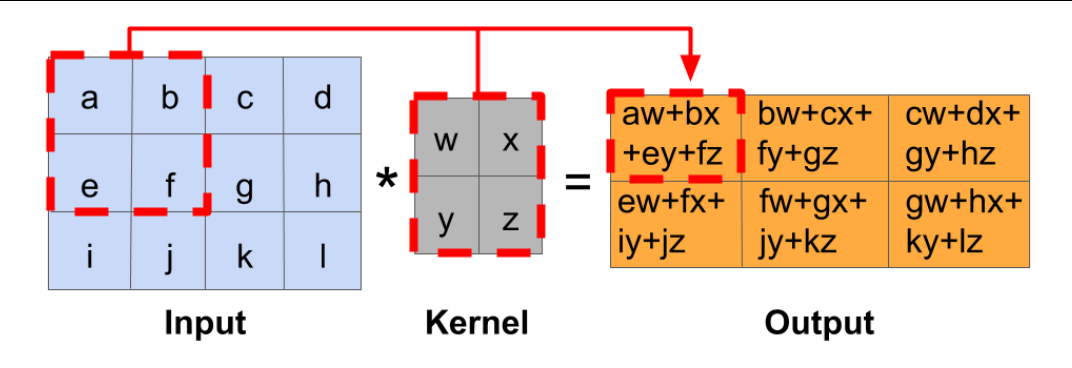
\includegraphics[width=0.7\textwidth]{images/arte/cnn1}
	\caption{Ejemplo de una convolución de dos dimensiones. Fuente \cite{temariodeeplearning}}
	\label{fig:cnn1}
\end{figure}


TODO Reduccion dimensión padding...

El proceso explicado anteriormente correspondería con una capa convolucional, que son el corazón de las redes neuronales convolucionales, sin embargo, en una red neuronal convolucional estas capas coexisten con otro tipo de capas que nos ayudaran a mejorar nuestros modelos. Las más usuales son:

\begin{itemize}
	\item Capa de agrupamiento (\textit{polling} en inglés): El objetivo de esta capa es agrupar un conjunto de salidas para obtener un único valor, al conjunto de valores de entrada (seleccionado de nuevo con un filtro) se le aplica una función para obtener un único valor. Aunque se pueden utilizar diferentes funciones, como puede ser la media, lo más usual es aplicar la función de máximo (\textit{max-polling}). Es habitual, intuir que usando esta función nos estamos quedando con las características más relevantes de cada cuadrante (del tamaño del filtro) de la entrada.
	\item Capa totalmente conectada: Hemos visto ejemplos de capas totalmente conectada al introducir las redes neuronales, esta capas usualmente se usan al final de nuestra red para tareas de clasificación, teniendo la última capa un número de neuronas igual al número de clases que pretendemos clasificar.
	\item Capa RELU: Si observamos la descripción de la operación de convolución nos damos cuenta de que se trata de una operación totalmente lineal, es por ello que después de cada capa de convolución es usual agregar una capa no lineal (también llamada capa de activación). Aunque se pueden utilizar otras funciones como la tangente o la función sigmoide, lo más usual es utilizar la función RELU.
	
	\item Capa de Dropout: 
	
\end{itemize}

En una red neuronal convolucional normalmente coexisten otro tipo de



TODO seguir con pooling ...

Encontramos una explicación más profunda sobre las redes convolucionales y su uso general en \cite{temariodeeplearning}. Nosotros nos centraremos en tener una visión general de su aplicación al Procesamiento del Lenguaje Natural, que también puede ampliarse en \cite{goldberg_2017}.


TODO palabras

\subsubsection{Redes neuronales recurrentes}


TODO explicación pros y contras

\section{BigData y Fast Data}

El primer uso del término  \textit{Big Data}  se da en un artículo de Michael Cox y David Ellsworth de la NASA publicado en 1997 (\cite{Cox_1997}), donde hacen referencia a la dificultad de procesar grandes volúmenes de datos con los métodos de la época. Sin embargo, fue en 2001 cuando encontramos la definición más conocida y aceptada de \textit{Big Data} hecha por el analista Laney Douglas en su artículo ``3D Data Management: Controlling Data Volume, Velocity y Variety''(\cite{laneay_2013}) en el que se hacía referencia a las ya ``famosas'' tres \textit{V}s:

\begin{itemize}
	\item \textbf{V}olumen:  Cada vez los volúmenes de datos son mayores.
	\item \textbf{V}elocidad: Es cada vez mayor la velocidad con la que se generan los datos.  
	\item \textbf{V}ariedad: Dejamos de tener únicamente datos completamente estructurados para trabajar con datos no estructurados y/o  semi-estructurados. 
\end{itemize} 


Google, como es obvio, también  se enfrentó a un importante problema a la hora de procesar la ingente cantidad de datos que generaba día a día y que no podían ser procesados de manera eficiente con el \textit{software} existente, es por ello que en el año 2003 presenta en \cite{GFS} su  \textit{``Google File System''} (GFS) y un año después \textit{Map Reduce} \cite{MapReduce}, estas dos capas de almacenamiento y procesamiento distribuido dieron lugar al nacimiento de lo que hoy conocemos como \textit{\textbf{Big Data}}.

Sin embargo, estas aportaciones no empezaron a tomar una repercusión relevante fuera de Google hasta el nacimiento del \textit{framework} Hadoop en 2006, un ecosistema con una gran cantidad de servicios pero cuya base fue Map Reduce y HDFS (basado en GFS). La complejidad del ecosistema \textit{Hadoop} hizo que éste no empezara a aparecer en las mayoría de las empresas hasta la creación de la compañía \textit{Cloudera} en 2009, que empezó a empaquetar los diferentes componentes del ecosistema \textit{Hadoop}, ofreciendo distribuciones estables y soporte para sus clientes. 

Durante estos 10 años la popularidad de \textit{Hadoop} ha crecido exponencialmente y junto con las BBDD NoSQL, nacidas también a partir de Google con su BigTable, forman lo que hoy conocemos como Big Data. 



El auge del \textbf{Big Data} ha llevado a algunas empresas a tener verdadera obsesión por el almacenamiento de todos los datos de sus clientes y las operaciones realizadas, creando inmensos \textit{datalakes} donde tener enormes históricos de todos sus datos, este ``síndrome de Diógenes digital'' creado por falsas expectativas, por la imposibilidad de extraer valor de los datos o por la dimensión cambiante de las empresas actuales, en la que los datos de años atrás pueden no ser relevantes en el presente, es uno de los posibles motivos por lo que el tratamiento de los datos esta cambiando. Otro de los motivos para el cambio de rumbo del \textit{Big Data} está relacionado con la \textit{V} de Velocidad, hoy en día no solo es importante la capacidad de ingestar rápidamente los datos, sino la capacidad de poder procesar y obtener decisiones o actuar en tiempo real a partir de los datos, aportando valor al negocio. En este escenario se vuelve más importante la velocidad que el volumen de datos, esto es lo que se denomina \textit{Fast Data}. 

Dentro del \textit{Fast Data} es habitual el uso de BBDD \textit{in-memory}, de buses de eventos y de tecnologías de procesamiento capaces de procesar los eventos en tiempo real. Como veremos posteriormente al desarrollar nuestra arquitectura, el \textit{Fast Data} será una parte fundamental en nuestro proyecto en el que tendremos que clasificar las llamadas en tiempo real y tomar decisiones (o alarmar) en función de las mismas.

%\chapter{Arquitectura y tecnologías}
\label{chapter:arquitectura}

El objetivo de este capítulo es tener un diseño esquemático de la solución que se plantée, este diseño será abordado en primer lugar desde un punto de vista lógico, de acuerdo a las necesidades del proyecto, posteriormente aterrizaremos esta arquitectura con tecnologías concretas que nos ayuden a conseguir el objetivo deseado.

\section{Arquitectura}
\begin{figure}[!ht]
	\centering
	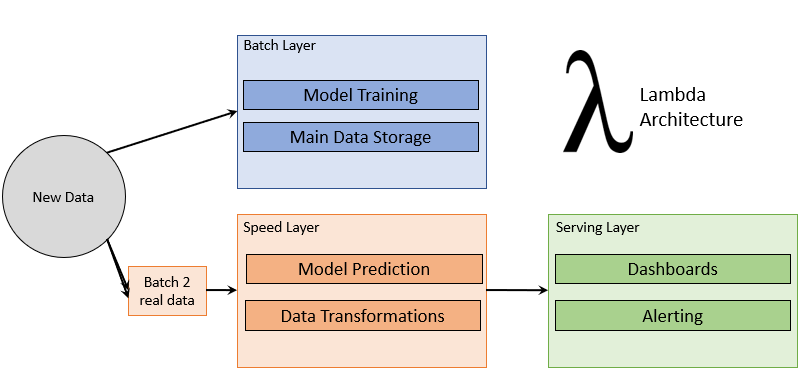
\includegraphics[width=1\textwidth]{images/arqu/lambda}
	\caption{Arquitectura Lambda propuesta}
	\label{fig:lambda}
\end{figure}




En este apartado definiremos la arquitectura desde un punto de vista lógico, esta arquitectura debe responder a los objetivos propuestos para cumplir con las necesidades de negocio existentes. 


En líneas generales, podemos ver la arquitectura de nuestro sistema como una arquitectura \textit{Lambda} en la que disponemos de una capa \textit{batch}, una capa rápida o \textit{real-time} y una última capa de servicio.



La capa batch será la encargada de entrenar el modelo a través de los datos de las llamadas, la capa rápida obtendrá los \textit{topics} de las llamadas en tiempo real usando el modelo previamente entrenado y por último la capa de servicio será la encargada de mostrar estos datos al usuario mediante cuadros de mando.  

En la figura \ref{fig:lambda} podemos ver un esquema general de nuestra arquitectura. A continuación definimos con más detalle cada una de las capas del modelo.




\subsection{Capa Batch}
El \textit{core} del proyecto que abordamos es el modelo, encargado de extraer los \textit{topics} de las transcripciones de llamadas al servicio de atención al cliente. Este modelo debe entrenarse usando un histórico suficientemente amplio. 

El modelo es un elemento vivo en nuestra arquitectura y, además de por posibles mejoras en los hiperparámetros o por la tecnología, debe re-entrenarse conforme se vayan recibiendo datos nuevos en el histórico, ya que es lógico pensar que la temática de las consultas variarán a lo largo del tiempo debido por ejemplo al lanzamiento de nuevos productos. 


\subsection{Capa Real-Time}
La \textit{speed layer} de nuestro proyecto será la encargada de recibir los datos en tiempo real, las llamadas serán publicadas en un bus de eventos y estos eventos serán consumidos por una capa de procesamiento que será la encargada de aplicar el modelo entrenado en la capa \textit{batch} a los nuevos datos. Los \textit{topics} resultantes de cada llamada serán publicados de nuevo en este bus para poder ser ingestados posteriormente a una BBDD NO-SQL, que será la encargada de proporcionar la información a la capa de servicio. 

Aprovecharemos también las características de la BBDD NoSQL para, mediante un módulo de \textit{Machine Learning}, detectar anomalías en series temporales y poder alarmar en el caso de que un \textit{topic} concreto se dispare en algún momento.  

Debido a la situación actual, las llamadas no se ingestan en \textit{real-time} si no que se procesan en mini \textit{batches} cada cierto tiempo. Es muy probable que este escenario cambie en el futuro por lo que se construirá un elemento de entrada a la capa rápida que transformará el mini-batch en eventos conforme vayan ejecutándose (este elemento puede observarse en la figura \ref{fig:lambda} como \textit{Batch 2 real data}). Esta pieza será suprimida una vez las llamadas sean recibidas en tiempo real. 


\subsection{Capa de Servicio}
Una vez almacenados los datos en la BBDD debemos construir un frontal que muestre al usuario el número de llamadas analizadas, el modelo utilizado y principalmente la evolución de los \textit{topics} a lo largo del tiempo. 

Lo ideal es que esta capa de servicio se vaya actualizando en tiempo cuasi-real y permita a los diferentes usuarios realizar cuadros de mando personalizados según sus necesidades. 

Otro requisito esencial en este tipo de proyectos es que la información este disponible vía API-REST para poder ser consumida por terceros.    


\section{Integración y Despliegue Continuos}
Como ya hemos visto al hablar del entrenamiento del modelo, el desarrollo de este tipo de proyectos no tiene un principio y un final, si no que se trata de un proceso cíclico en el que por necesidades del negocio, por cambio en los datos o por cambio en la tecnologías, será necesario añadir mejoras o modificaciones en nuestro desarrollo. 

Por estos motivos es conveniente definir mecanismos que nos permitan, tras cada cambio efectuado, poder realizar las pruebas necesarias y desplegar estos cambios de una manera totalmente automatizada y sin intervención del usuario. 

Aunque este apartado queda fuera de la implementación inicial del proyecto es imprescindible llevarlo a cabo para que este sea sostenible a lo largo del tiempo. 


TODO (Posible ampliar con apuntes sobre el ciclo de vida de los datos y contar beneficios de un despliegue continuo)

\section{Tecnologías}

Al igual que la arquitectura descrita anteriormente era la encargada de responder a las necesidades de negocio, las tecnologías descritas en este apartado nos darán las piezas necesarias para poder construir esa arquitectura y dar respuesta a nuestro caso de uso. 


En el proceso de selección de las tecnologías, no solo se ha tenido en cuenta la idoneidad de las mismas para el caso de uso, si no que se ha valorado también la experiencia en la misma y la disponibilidad dentro del entorno de trabajo. Esto puede provocar que en algunos casos aunque la tecnología se adapte al caso de uso, puedan existir otras soluciones más óptimas cuyo uso era menos viable dado los plazos de ejecución del proyecto. 

A continuación enumeraremos las tecnologías agrupadas en las diferentes capas que hemos comentado en el apartado de arquitectura, además añadiremos las tecnologías que se usarán para la integración y despliegue continuo. 

\subsection{Capa batch}

\begin{itemize}
	\item \textbf{Spark}: Es un framework de computación en clúster. Este \textit{framework} se encuentra desplegado sobre un clúster Hadoop, específicamente una distribución HortonWorks, y posee librerías específicas para Machine Learning como MLLIB.
	\item \textbf{Tensorflow} sobre GPUs: Para el entrenamiento de los modelos también disponemos de un cluster con GPUs sobre el que podremos correr código usando la librería de Google Tensorflow para entrenar nuestros modelos.
\end{itemize}

\subsection{Capa Real-Time}

\begin{itemize}
	\item \textbf{Kafka}: Es el \textit{core} de la capa rápida, se trata de un bus de evento distribuido a través del cual se realizara la ingesta o publicación de los eventos (llamadas). Las diferentes capas de procesamiento que requieran estos eventos se suscribirán a este Bus.
	\item \textbf{Microservicios}: En nuestra capa Real Time construiremos diferentes microservicios en la capa de procesamiento, estos microservicios serán por ejemplo los encargados de devolver los \textit{topics} de cada llamada a partir de una llamada API REST. Estos microservicios correran sobre contenedores en una plataforma Openshift. 
	\item\textbf{ Kafka Stream y KSQL}: A la hora de procesar la información en eventos ingestada en nuestro Bus Kafka disponemos de dos herramientas muy potentes que son Kafka Stream y KSQL. El primero consiste en una serie de librerías que nos permiten construir aplicaciones y microservicios cuyo origen y destino sean un Bus Kafka. KSQL en cambio es un motor SQL aplicable a eventos que nos llegan mediante \textit{streaming}.
	\item \textbf{Logstash}: Una vez hayamos extraído los \textit{topics} correspondientes a cada llamada o evento, tendremos que ingestar esta información en nuestra BBDD, que en este caso será Elasticsearch. Logstash nos permitirá leer de Kafka, realizar las transformaciones necesarias y volcar la información resultante en Elasticsearch.
	\item \textbf{Elasticsearch}: Aunque no se trata en el sentido más estricto de una BBDD No-SQL, si no de un motor de búsqueda, Elasticsearch nos permite almacenar la información en forma de documentos json y realizar consultas y agregaciones sobre cualquier campo. Entre las características que podemos aprovechar de Elasticsearch para nuestro objetivo están: 
	\begin{itemize}
		\item Ingesta en tiempo casi real.
		\item Consulta en tiempo casi real. 
		\item Disponibilidad de mecanismos de ingesta (Logstash) y consulta (kibana).
		\item Posibilidad de crear alarmas en base a consultas. 
		\item Posibilidad de crear \textit{jobs} de Machine Learning que detecten anomalías en series temporales. 
	\end{itemize}
	
	
\end{itemize}

\subsection{Capa Servicio}
\begin{itemize}
	\item \textbf{Elasticsearch API REST}: Toda la información almacenada previamente en Elasticsearch puede ser accedida a través de su API REST por lo que será nuestro método de publicación de la información. 
	\item \textbf{Kibana}: Será el frontal donde los usuarios podrán consultar sus diferentes cuadros de mando y construir nuevos de acuerdo a sus necesidades. También, gracias al modulo de \textit{machine learning} de Elasticsearch, los usuarios podrán crear \textit{jobs} de \textit{machine learning} para detectar anomalías en los temas tratados y generar las alertas necesarias.
\end{itemize}


\subsection{Integración y Despliegue Continuo}
Aunque la implementación de esta parte se escapa de los plazos del proyecto, las tecnologías que se usarán para llevarla a cabo serán. 
\begin{itemize}
	\item \textbf{BitBucket}: Será el repositorio usado para almacenar las nuevas versiones de nuestro \textit{software} de manera que podamos tener un control de versiones.
	\item \textbf{Jenkins}: Es un servidor de integración continua \textit{open source}  que mediante la creación de tareas nos ayudará a realizar el \textit{build} de nuestro software realizando de manera automática las pruebas necesarias.
\end{itemize}
%\chapter{Conjunto de datos}
\label{chapter:dataset}
El primer paso cuando nos enfrentamos a un problema de minería de datos es comprender los datos con los que contamos y ver si se adaptan a nuestras necesidades. En este caso, al tratarse de un proyecto que se realiza dentro de una empresa, tenemos la posibilidad de acudir a las áreas dueñas del dato para solicitarle información adicional sobre el mismo. 

En este apartado haremos un recorrido 



\section{Evolución del \textit{dataset}}

\subsection{Las llamadas}

Durante este apartado hemos realizado un análisis del conjunto de datos más completo que teníamos hasta la fecha, no obstante, el proceso para conseguir y entender este conjunto de datos no ha sido una tarea trivial sino que se ha tratado de un proceso iterativo en el que ha sido necesario involucrar a varias áreas y extraer información de diversas fuentes de datos de la compañía. Estos datos, como veremos de nuevo en el siguiente capítulo, nos han llevado a crear modelos poco eficientes que nos han situado otra vez en el punto de partida. 

Aunque el hecho de volver a la fase de recopilación y entendimiento de los datos es algo que ya preveíamos cuando presentamos el estándar \textbf{\textit{CRISP-DM}} (apartado \ref{section:intro:planificacion}) vamos a utilizar esta sección una breve muestra de los análisis iniciales para que pueda compararse con el análisis final y quede patente la evolución de los datos.



Este análisis fue realizado en \textit{PySpark} y el primer paso, como es obvio, fue cargar los datos en un \textit{dataframe} y comprobar la estructura del mismo: 


\vspace{0.5cm}

\begin{tcolorbox}[breakable, size=fbox, boxrule=1pt, pad at break*=1mm,colback=cellbackground, colframe=cellborder]
\prompt{In}{incolor}{1}{\boxspacing}
\begin{Verbatim}[commandchars=\\\{\}]
\PY{n}{domo\PYZus{}dataset} \PY{o}{=} \PY{n}{sqlContext}\PY{o}{.}\PY{n}{read}\PY{o}{.}\PY{n}{parquet}\PY{p}{(}\PY{l+s+s2}{\PYZdq{}}\PY{l+s+s2}{dataset/domo\PYZus{}dataset.parquet}\PY{l+s+s2}{\PYZdq{}}\PY{p}{)}
\PY{n}{domo\PYZus{}dataset}
\end{Verbatim}
\end{tcolorbox}

 \begin{tcolorbox}[breakable, size=fbox, boxrule=.5pt, pad at break*=1mm, opacityfill=0]
\prompt{Out}{outcolor}{1}{\boxspacing}
\begin{Verbatim}[commandchars=\\\{\}]
DataFrame[co\_llamada\_verint: string, id\_descarga:string,nu\_telefono\_actuacion:string, it\_llamada: timestamp, nu\_llamada\_ic: string, co\_grabacion: string,raw\_verint:array<string>, \_\_index\_level\_0\_\_: bigint]
\end{Verbatim}
\end{tcolorbox}


De los campos listados unicamente es factible extraer información del texto de la llamada (``raw\_verint''). El siguiente paso fue comprobar el número de llamadas que no contenían una transcripción nula. Además reparticionamos los datos y los dejamos en caché para realizar un análisis más eficiente: 

\vspace{0.5cm}


    \begin{tcolorbox}[breakable, size=fbox, boxrule=1pt, pad at break*=1mm,colback=cellbackground, colframe=cellborder]
\prompt{In}{incolor}{2}{\boxspacing}
\begin{Verbatim}[commandchars=\\\{\}]
\PY{n}{raw\PYZus{}verint} \PY{o}{=} \PY{n}{domo\PYZus{}dataset}\PY{o}{.}\PY{n}{select}\PY{p}{(}\PY{l+s+s2}{\PYZdq{}}\PY{l+s+s2}{raw\PYZus{}verint}\PY{l+s+s2}{\PYZdq{}}\PY{p}{)}\PY{o}{.}\PY{n}{rdd}\PY{o}{.}\PY{n}{filter}\PY{p}{(}\PY{k}{lambda} \PY{n}{x}\PY{p}{:} \PY{n}{x}\PY{p}{[}\PY{l+s+s2}{\PYZdq{}}\PY{l+s+s2}{raw\PYZus{}verint}\PY{l+s+s2}{\PYZdq{}}\PY{p}{]} \PY{o+ow}{is} \PY{o+ow}{not} \PY{k+kc}{None}\PY{p}{)}\PYZbs{}
    \PY{o}{.}\PY{n}{map}\PY{p}{(}\PY{k}{lambda} \PY{n}{x}\PY{p}{:} \PY{l+s+s2}{\PYZdq{}}\PY{l+s+s2}{ }\PY{l+s+s2}{\PYZdq{}}\PY{o}{.}\PY{n}{join}\PY{p}{(}\PY{n+nb}{map}\PY{p}{(}\PY{k}{lambda} \PY{n}{y}\PY{p}{:} \PY{l+s+s2}{\PYZdq{}}\PY{l+s+s2}{ }\PY{l+s+s2}{\PYZdq{}}\PY{o}{.}\PY{n}{join}\PY{p}{(}\PY{n}{y}\PY{p}{)}\PY{p}{,} \PY{n}{x}\PY{p}{)}\PY{p}{)}\PY{p}{)}\PYZbs{}
    \PY{o}{.}\PY{n}{repartition}\PY{p}{(}\PY{l+m+mi}{17}\PY{p}{)}
\PY{n}{raw\PYZus{}verint}\PY{o}{.}\PY{n}{cache}\PY{p}{(}\PY{p}{)}
\PY{n+nb}{print}\PY{p}{(}\PY{l+s+s1}{\PYZsq{}}\PY{l+s+s1}{Llamadas disponibles : }\PY{l+s+si}{\PYZob{}:,\PYZcb{}}\PY{l+s+s1}{\PYZsq{}}\PY{o}{.}\PY{n}{format}\PY{p}{(} \PY{n}{raw\PYZus{}verint}\PY{o}{.}\PY{n}{count}\PY{p}{(}\PY{p}{)}\PY{p}{)}\PY{p}{)}  
\end{Verbatim}
\end{tcolorbox}

    \begin{Verbatim}[commandchars=\\\{\}]
Llamadas disponibles : 185,109
    \end{Verbatim}
    
    
 A través de todas las llamadas obtuvimos una lista de palabras: 
    \vspace{0.5cm}
    
        \begin{tcolorbox}[breakable, size=fbox, boxrule=1pt, pad at break*=1mm,colback=cellbackground, colframe=cellborder]
    \prompt{In}{incolor}{3}{\boxspacing}
    \begin{Verbatim}[commandchars=\\\{\}]
    \PY{n}{raw\PYZus{}list\PYZus{}word} \PY{o}{=} \PY{n}{raw\PYZus{}verint}\PY{o}{.}\PY{n}{map}\PY{p}{(} \PY{k}{lambda} \PY{n}{document}\PY{p}{:} \PY{n}{document}\PY{o}{.}\PY{n}{strip}\PY{p}{(}\PY{p}{)}\PY{o}{.}\PY{n}{lower}\PY{p}{(}\PY{p}{)}\PY{p}{)} \PYZbs{}
                    \PY{o}{.}\PY{n}{map}\PY{p}{(} \PY{k}{lambda} \PY{n}{document}\PY{p}{:} \PY{n}{re}\PY{o}{.}\PY{n}{split}\PY{p}{(}\PY{l+s+s2}{\PYZdq{}}\PY{l+s+s2}{ }\PY{l+s+s2}{\PYZdq{}}\PY{p}{,} \PY{n}{document}\PY{p}{)}\PY{p}{)}
    
    \PY{n}{raw\PYZus{}list\PYZus{}word}\PY{o}{.}\PY{n}{take}\PY{p}{(}\PY{l+m+mi}{1}\PY{p}{)}
    \end{Verbatim}
    \end{tcolorbox}
    
    
    
Y eliminamos las \textit{Stopwords} en español usando el paquete \textit{ntlk}.

\vspace{0.5cm}
    
        \begin{tcolorbox}[breakable, size=fbox, boxrule=1pt, pad at break*=1mm,colback=cellbackground, colframe=cellborder]
    \prompt{In}{incolor}{4}{\boxspacing}
    \begin{Verbatim}[commandchars=\\\{\}]
    \PY{n}{StopWords} \PY{o}{=} \PY{n}{stopwords}\PY{o}{.}\PY{n}{words}\PY{p}{(}\PY{l+s+s2}{\PYZdq{}}\PY{l+s+s2}{spanish}\PY{l+s+s2}{\PYZdq{}}\PY{p}{)}
    
    \PY{n}{raw\PYZus{}no\PYZus{}stop} \PY{o}{=} \PY{n}{raw\PYZus{}verint}\PY{o}{.}\PY{n}{map}\PY{p}{(} \PY{k}{lambda} \PY{n}{document}\PY{p}{:} \PY{n}{document}\PY{o}{.}\PY{n}{strip}\PY{p}{(}\PY{p}{)}\PY{o}{.}\PY{n}{lower}\PY{p}{(}\PY{p}{)}\PY{p}{)} \PYZbs{}
    	\PY{o}{.}\PY{n}{map}\PY{p}{(} \PY{k}{lambda} \PY{n}{document}\PY{p}{:} \PY{n}{re}\PY{o}{.}\PY{n}{split}\PY{p}{(}\PY{l+s+s2}{\PYZdq{}}\PY{l+s+s2}{ }\PY{l+s+s2}{\PYZdq{}}\PY{p}{,} \PY{n}{document}\PY{p}{)}\PY{p}{)} \PYZbs{}
        \PY{o}{.}\PY{n}{map}\PY{p}{(} \PY{k}{lambda} \PY{n}{word}\PY{p}{:} \PY{p}{[}\PY{n}{x} \PY{k}{for} \PY{n}{x} \PY{o+ow}{in} \PY{n}{word} \PY{k}{if} \PY{n}{x} \PY{o+ow}{not} \PY{o+ow}{in} \PY{n}{StopWords}\PY{p}{]}\PY{p}{)}
    \PY{n}{raw\PYZus{}no\PYZus{}stop}\PY{o}{.}\PY{n}{take}\PY{p}{(}\PY{l+m+mi}{1}\PY{p}{)}
    \end{Verbatim}
    \end{tcolorbox}
    
       Volvemos a unir las palabras de la lista (ahora sin las \textit{stopwords}) para mostrar una nube de  palabras más frecuentes
    
        \begin{tcolorbox}[breakable, size=fbox, boxrule=1pt, pad at break*=1mm,colback=cellbackground, colframe=cellborder]
    \prompt{In}{incolor}{5}{\boxspacing}
    \begin{Verbatim}[commandchars=\\\{\}]
    \PY{n}{list\PYZus{}words} \PY{o}{=} \PY{n}{raw\PYZus{}no\PYZus{}stop}\PY{o}{.}\PY{n}{reduce}\PY{p}{(}\PY{k}{lambda} \PY{n}{a}\PY{p}{,}\PY{n}{b}\PY{p}{:} \PY{n+nb}{list}\PY{p}{(}\PY{n+nb}{set}\PY{p}{(}\PY{n}{a}\PY{o}{+}\PY{n}{b}\PY{p}{)}\PY{p}{)}\PY{p}{)}  
    \PY{n}{wordcloud} \PY{o}{=} \PY{n}{WordCloud}\PY{p}{(}\PY{p}{)}\PY{o}{.}\PY{n}{generate}\PY{p}{(}\PY{l+s+s2}{\PYZdq{}}\PY{l+s+s2}{ }\PY{l+s+s2}{\PYZdq{}}\PY{o}{.}\PY{n}{join}\PY{p}{(}\PY{n}{list\PYZus{}words}\PY{p}{)}\PY{p}{)}
    \PY{n}{plt}\PY{o}{.}\PY{n}{figure}\PY{p}{(}\PY{n}{figsize} \PY{o}{=} \PY{p}{(}\PY{l+m+mi}{20}\PY{p}{,}\PY{l+m+mi}{20}\PY{p}{)}\PY{p}{)}
    \PY{n}{plt}\PY{o}{.}\PY{n}{imshow}\PY{p}{(}\PY{n}{wordcloud}\PY{p}{,} \PY{n}{interpolation}\PY{o}{=}\PY{l+s+s1}{\PYZsq{}}\PY{l+s+s1}{bilinear}\PY{l+s+s1}{\PYZsq{}}\PY{p}{)}
    \PY{n}{plt}\PY{o}{.}\PY{n}{axis}\PY{p}{(}\PY{l+s+s2}{\PYZdq{}}\PY{l+s+s2}{off}\PY{l+s+s2}{\PYZdq{}}\PY{p}{)}
    \PY{n}{plt}\PY{o}{.}\PY{n}{show}\PY{p}{(}\PY{p}{)}
    \end{Verbatim}
    \end{tcolorbox}
    
      \begin{figure}[!ht]
                    	\centering
                    	\adjustimage{max size={0.9\linewidth}{0.9\paperheight}}{images/data/malo_wordclod1}
                    	\caption{Primeros datos: \textit{wordcloud} inicial}
                    	\label{fig:wordcloudmalo1}
                    \end{figure}
              
              
Como podemos observar en la nube de palabras obtenida, el resultado no fue el esperado. Las llamadas que aparecían no eran significante y entre ellas existían muchas malas  transcripciones. A partir de aquí intentamos abordar distintas aproximaciones que nos permitieran poder extraer algo de valor de los datos.

Un ejemplo de estas aproximaciones fue \textit{taggear} las palabras en  función de su categoría gramatical para quedarnos solo con una lista de candidatos. Para hacerlo de un modo eficiente de manera distribuida en promer lugar creamos un diccionario con las categorías y la raíz de las palabras: 

          
\vspace{0.5cm}
          
              \begin{tcolorbox}[breakable, size=fbox, boxrule=1pt, pad at break*=1mm,colback=cellbackground, colframe=cellborder]
          \prompt{In}{incolor}{6}{\boxspacing}
          \begin{Verbatim}[commandchars=\\\{\}]
          \PY{n}{tagger} \PY{o}{=} \PY{n}{treetaggerwrapper}\PY{o}{.}\PY{n}{TreeTagger}\PY{p}{(}\PY{n}{TAGLANG}\PY{o}{=}\PY{l+s+s1}{\PYZsq{}}\PY{l+s+s1}{es}\PY{l+s+s1}{\PYZsq{}}\PY{p}{,} \PY{n}{TAGPARFILE}\PY{o}{=}\PY{l+s+s2}{\PYZdq{}}\PY{l+s+s2}{/tmp/tree/spanish.par}\PY{l+s+s2}{\PYZdq{}}\PY{p}{,} \PY{n}{TAGDIR}\PY{o}{=}\PY{l+s+s2}{\PYZdq{}}\PY{l+s+s2}{/tmp/tree/tree\PYZhy{}tagger\PYZhy{}3.2.1/}\PY{l+s+s2}{\PYZdq{}}\PY{p}{)}          
          \PY{n}{vocabulary} \PY{o}{=}  \PY{n}{raw\PYZus{}no\PYZus{}stop}\PY{o}{.}\PY{n}{filter}\PY{p}{(}\PY{k}{lambda} \PY{n}{x}\PY{p}{:} \PY{n+nb}{len}\PY{p}{(}\PY{n}{x}\PY{p}{)}\PY{o}{\PYZgt{}}\PY{l+m+mi}{0}\PY{p}{)} \PYZbs{}
              \PY{o}{.}\PY{n}{flatMap}\PY{p}{(}\PY{k}{lambda} \PY{n}{document}\PY{p}{:} \PY{n}{document}\PY{p}{)} \PYZbs{}
              \PY{o}{.}\PY{n}{map}\PY{p}{(}\PY{k}{lambda} \PY{n}{word}\PY{p}{:} \PY{p}{(}\PY{n}{word}\PY{p}{,} \PY{l+m+mi}{1}\PY{p}{)}\PY{p}{)} \PYZbs{}
              \PY{o}{.}\PY{n}{reduceByKey}\PY{p}{(} \PY{k}{lambda} \PY{n}{x}\PY{p}{,}\PY{n}{y}\PY{p}{:} \PY{n}{x} \PY{o}{+} \PY{n}{y}\PY{p}{)}   \PYZbs{}
              \PY{o}{.}\PY{n}{map}\PY{p}{(}\PY{k}{lambda} \PY{n+nb}{tuple}\PY{p}{:} \PY{n+nb}{tuple}\PY{p}{[}\PY{l+m+mi}{0}\PY{p}{]}\PY{p}{)} 
          \PY{n}{vocabulary}\PY{o}{.}\PY{n}{cache}\PY{p}{(}\PY{p}{)}
          \PY{n}{vocabulary}\PY{o}{.}\PY{n}{count}\PY{p}{(}\PY{p}{)}
          \PY{n}{vocabulary\PYZus{}tags} \PY{o}{=} \PY{n+nb}{list}\PY{p}{(}\PY{n+nb}{map}\PY{p}{(}\PY{k}{lambda} \PY{n}{el}\PY{p}{:} \PY{p}{(}\PY{n}{el}\PY{p}{[}\PY{l+m+mi}{0}\PY{p}{]}\PY{p}{,} \PY{p}{(}\PY{n}{el}\PY{p}{[}\PY{l+m+mi}{1}\PY{p}{]}\PY{p}{,} \PY{n}{el}\PY{p}{[}\PY{l+m+mi}{2}\PY{p}{]}\PY{p}{)} \PY{p}{)} \PY{p}{,}\PY{n+nb}{map}\PY{p}{(}\PY{k}{lambda} \PY{n}{y}\PY{p}{:} \PY{n}{y}\PY{o}{.}\PY{n}{split}\PY{p}{(}\PY{l+s+s2}{\PYZdq{}}\PY{l+s+se}{\PYZbs{}t}\PY{l+s+s2}{\PYZdq{}}\PY{p}{)}\PY{p}{,}\PY{n+nb}{list}\PY{p}{(}\PY{n}{tagger}\PY{o}{.}\PY{n}{tag\PYZus{}text}\PY{p}{(}\PY{p}{(}\PY{l+s+s2}{\PYZdq{}}\PY{l+s+s2}{ }\PY{l+s+s2}{\PYZdq{}}\PY{o}{.}\PY{n}{join}\PY{p}{(}\PY{n}{vocabulary}\PY{o}{.}\PY{n}{collect}\PY{p}{(}\PY{p}{)}\PY{p}{)}\PY{p}{)} \PY{p}{)}\PY{p}{)}\PY{p}{)}\PY{p}{)}\PY{p}{)}
          \PY{n}{tags\PYZus{}dict} \PY{o}{=} \PY{n}{sc}\PY{o}{.}\PY{n}{broadcast}\PY{p}{(}\PY{p}{\PYZob{}}\PY{n}{key}\PY{p}{:} \PY{n}{value} \PY{k}{for} \PY{p}{(}\PY{n}{key}\PY{p}{,} \PY{n}{value}\PY{p}{)} \PY{o+ow}{in} \PY{n}{vocabulary\PYZus{}tags}\PY{p}{\PYZcb{}}\PY{p}{)}
          \end{Verbatim}
          \end{tcolorbox}
          
             Una vez que hemos filtrado nos quedamos unicamente con la raíz de las palabras que sean
          verbos o nombres.
          
          \vspace{0.5cm}
          
              \begin{tcolorbox}[breakable, size=fbox, boxrule=1pt, pad at break*=1mm,colback=cellbackground, colframe=cellborder]
          \prompt{In}{incolor}{7}{\boxspacing}
          \begin{Verbatim}[commandchars=\\\{\}]
          \PY{k}{def} \PY{n+nf}{get\PYZus{}stem\PYZus{}of\PYZus{}candidates}\PY{p}{(}\PY{n}{x}\PY{p}{)}\PY{p}{:}
              \PY{n}{good} \PY{o}{=} \PY{p}{[}\PY{l+s+sa}{u}\PY{l+s+s1}{\PYZsq{}}\PY{l+s+s1}{VLinf}\PY{l+s+s1}{\PYZsq{}}\PY{p}{,} \PY{l+s+sa}{u}\PY{l+s+s1}{\PYZsq{}}\PY{l+s+s1}{NC}\PY{l+s+s1}{\PYZsq{}}\PY{p}{]}
              \PY{n}{candidates} \PY{o}{=}  \PY{n+nb}{list}\PY{p}{(}\PY{n+nb}{filter}\PY{p}{(}\PY{k}{lambda} \PY{n}{word}\PY{p}{:} \PY{n}{word} \PY{o+ow}{in} \PY{n}{tags\PYZus{}dict}\PY{o}{.}\PY{n}{value} \PY{o+ow}{and} \PY{n}{tags\PYZus{}dict}\PY{o}{.}\PY{n}{value}\PY{p}{[}\PY{n}{word}\PY{p}{]}\PY{p}{[}\PY{l+m+mi}{0}\PY{p}{]} \PY{o+ow}{in} \PY{n}{good}  \PY{p}{,}\PY{n}{x}\PY{p}{)}\PY{p}{)}
              \PY{n}{stem} \PY{o}{=} \PY{n+nb}{list}\PY{p}{(}\PY{n+nb}{map}\PY{p}{(}\PY{k}{lambda} \PY{n}{word}\PY{p}{:} \PY{n}{tags\PYZus{}dict}\PY{o}{.}\PY{n}{value}\PY{p}{[}\PY{n}{word}\PY{p}{]}\PY{p}{[}\PY{l+m+mi}{1}\PY{p}{]}\PY{p}{,} \PY{n}{candidates}\PY{p}{)}\PY{p}{)}
              \PY{k}{return} \PY{n}{stem}
              
          \PY{n}{stemmed\PYZus{}candidates} \PY{o}{=} \PY{n}{raw\PYZus{}no\PYZus{}stop}\PY{o}{.}\PY{n}{map}\PY{p}{(}\PY{n}{get\PYZus{}stem\PYZus{}of\PYZus{}candidates}\PY{p}{)}    
          \PY{n}{stemmed\PYZus{}candidates}\PY{o}{.}\PY{n}{cache}\PY{p}{(}\PY{p}{)}
          \end{Verbatim}
          \end{tcolorbox}
         
         Con estos resultado volvemos a crear la nube de palabras.  
         
         \vspace{0.5cm}

                  
              \begin{tcolorbox}[breakable, size=fbox, boxrule=1pt, pad at break*=1mm,colback=cellbackground, colframe=cellborder]
          \prompt{In}{incolor}{8}{\boxspacing}
          \begin{Verbatim}[commandchars=\\\{\}]
          \PY{n}{list\PYZus{}stemmed\PYZus{}words} \PY{o}{=} \PY{n}{stemmed\PYZus{}candidates}\PY{o}{.}\PY{n}{reduce}\PY{p}{(}\PY{k}{lambda} \PY{n}{a}\PY{p}{,}\PY{n}{b}\PY{p}{:} \PY{n+nb}{list}\PY{p}{(}\PY{n+nb}{set}\PY{p}{(}\PY{n}{a}\PY{o}{+}\PY{n}{b}\PY{p}{)}\PY{p}{)}\PY{p}{)}
          
          \PY{n}{wordcloud} \PY{o}{=} \PY{n}{WordCloud}\PY{p}{(}\PY{p}{)}\PY{o}{.}\PY{n}{generate}\PY{p}{(}\PY{l+s+s2}{\PYZdq{}}\PY{l+s+s2}{ }\PY{l+s+s2}{\PYZdq{}}\PY{o}{.}\PY{n}{join}\PY{p}{(}\PY{n}{list\PYZus{}stemmed\PYZus{}words}\PY{p}{)}\PY{p}{)}
          
          \PY{c+c1}{\PYZsh{} Display the generated image:}
          \PY{n}{plt}\PY{o}{.}\PY{n}{figure}\PY{p}{(}\PY{n}{figsize} \PY{o}{=} \PY{p}{(}\PY{l+m+mi}{20}\PY{p}{,}\PY{l+m+mi}{20}\PY{p}{)}\PY{p}{)}
          
          \PY{n}{plt}\PY{o}{.}\PY{n}{imshow}\PY{p}{(}\PY{n}{wordcloud}\PY{p}{,} \PY{n}{interpolation}\PY{o}{=}\PY{l+s+s1}{\PYZsq{}}\PY{l+s+s1}{bilinear}\PY{l+s+s1}{\PYZsq{}}\PY{p}{)}
          \PY{n}{plt}\PY{o}{.}\PY{n}{axis}\PY{p}{(}\PY{l+s+s2}{\PYZdq{}}\PY{l+s+s2}{off}\PY{l+s+s2}{\PYZdq{}}\PY{p}{)}
          \PY{n}{plt}\PY{o}{.}\PY{n}{show}\PY{p}{(}\PY{p}{)}
          \end{Verbatim}
          \end{tcolorbox}
          
     
              
              \begin{figure}[!ht]
              	\centering
              	\adjustimage{max size={0.9\linewidth}{0.9\paperheight}}{images/data/malo_wordclod2}
                    	\caption{Primeros datos: \textit{wordcloud} filtrado}
                    	\label{fig:wordcloudmalo2}
              \end{figure}
              
              
              
              
 Observando que los resultados no mejoran con esta propuesta, tampoco lo hicieron con la obtención de N-Gramas, y en el capítulo siguiente veremos que la creación de los modelos sobre este conjunto de datos nos llevó a volver a buscar y entender nuevos datos.
 
 
 \subsection{Las etiquetas}
 
 Tras ver la pobre calidad de los datos iniciales, intentamos encontrar algún dato que nos sirviera para etiquetar las llamadas pensando que podrían ser de utilidad para un modelo supervisado. Una posibilidad era revisar e etiquetar llamadas manualmente, pero dado la cantidad de datos que podían ser necesarios para entrenar un modelo supervisado convertía esta posibilidad en inviable. 
 
 

% bibliografia
\addcontentsline{toc}{chapter}{Bibliografía}
\bibliographystyle{plain}
\nocite{*}
\bibliography{referencias}

\end{document}